\begin{frame}
	\frametitle{Atmosphäre - Luftmassen}

	\begin{figure}
		\centering
		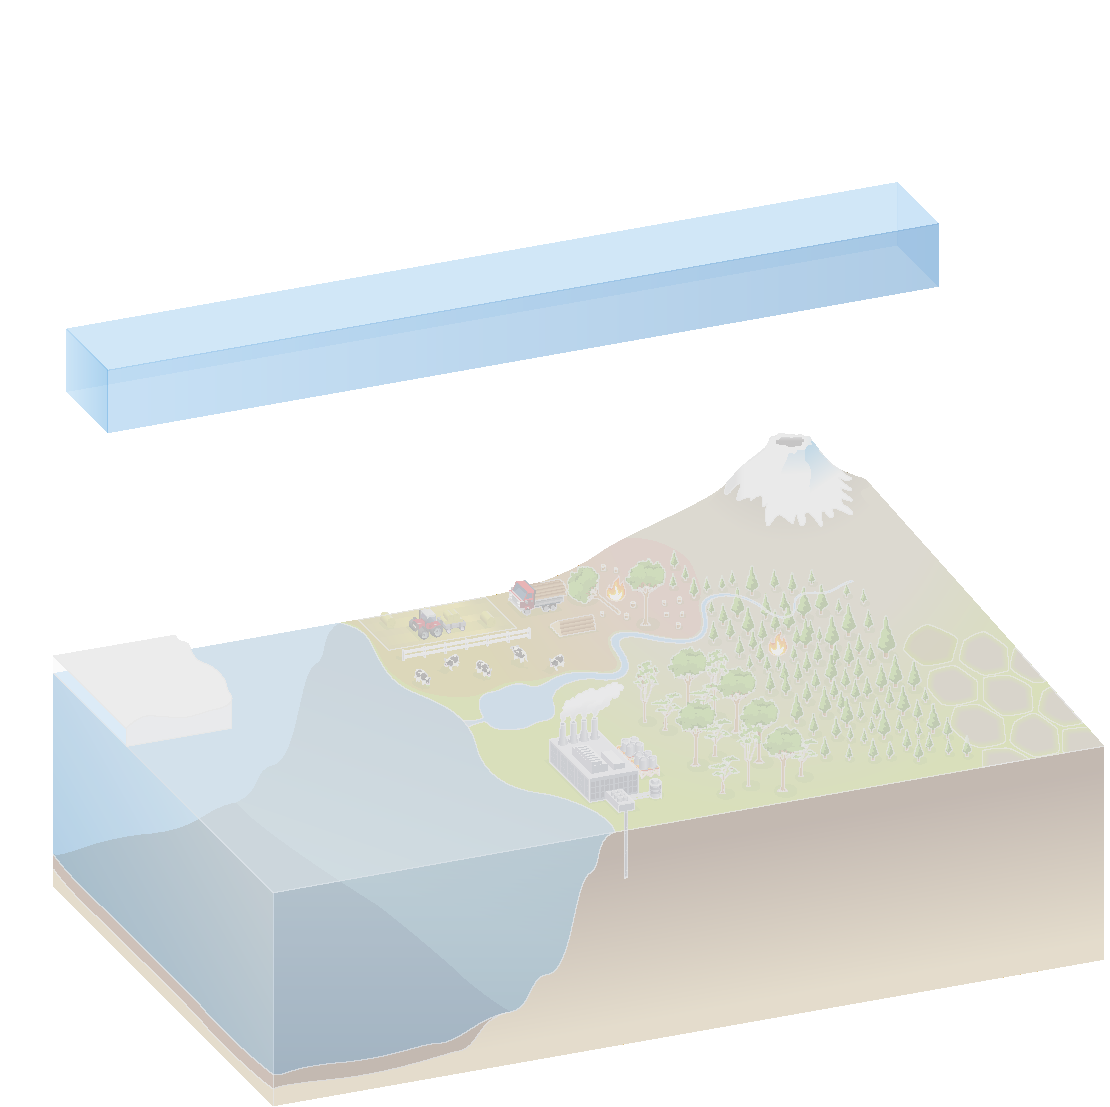
\includegraphics[trim={1cm 0cm 0cm 3cm}, clip, width=0.55\linewidth]{%
        bilder/climate_components/global_climate_components_atmosphere.pdf}
		\caption{Die Atmosphäre ist der Faktor des Klimasystems der am schnellsten auf Änderungen des Erdsystems reagiert.}
	\end{figure}

	\note{
		\begin{itemize}
			\item[] Luft
		\end{itemize}
	}
\end{frame}
